\documentclass[a4paper,titlepage]{scrartcl}
\pagestyle{plain}
\usepackage[utf8]{inputenc}
\usepackage[T1]{fontenc}
\usepackage[german]{babel}
\usepackage{float}
\usepackage{graphicx}
\usepackage{amsmath,amssymb,amstext}
\usepackage{enumerate}
\usepackage{units,url}
\usepackage{mhchem,numprint,multirow}
\renewcommand{\sc}{\textsc}

\numberwithin{equation}{section}

\title{Messung der Winkelkorrelation von $\gamma$-Strahlung}
\author{Genti Saliu, Jonas Müller\\Gruppe 106}
\date{Versuchstag: 19. November 2014}

\begin{document}
	\begin{titlepage}
		\maketitle
		\thispagestyle{empty}
	\end{titlepage}
	
\newpage
\pagenumbering{roman}
\tableofcontents

\newpage
\pagenumbering{arabic}

\section{Theoretische Grundlagen}
\subsection{Radioaktivität und Strahlungsarten \cite{wiki:radioactivity}}
Mit Radioaktivität bezeichnet man die Eigenschaft instabiler Atomkerne, sich spontan in anderen Atomkerne umzuwandeln und dabei ionisierende Strahlung auszusenden. Dieser Prozess wird anders auch als radioaktiver Zerfall oder Kernzerfall bezeichnet.\\ \\
Die in diesem Umwandlungsprozess frei werdende Energie wird in der Regel als $\alpha$-, $\beta$ oder $\gamma$-Strahlung emittiert, auf denen nachfolgend im Detail eingegangen wird. Jede dieser Strahlungsarten ist für den Menschen ab einer bestimmten Dosis gefährlich und nicht direkt wahrnehmbar. Nach einer für den radioaktiven Stoff charakteristischen Zeit, der \textbf{Halbwertszeit}, halbiert sich dessen Menge und somit auch dessen Aktivität und Strahlenemission. Die Halbwertszeit liegt im Bereich von Sekundenbruchteilen bis hin zu Trillionen Jahren.

\subsubsection{$\alpha$-Strahlung}
Beim Alpha-Zerfall zerfällt ein radioaktives Nuklid unter Aussendung eines Helium-4-Atomkerns ($\ce{^{4}He}$) in einen Kern mit Ordnungszahl $Z-2$ und Massenzahl $A-4$.
\begin{equation*}
\ce{^{A}_{Z}X} \rightarrow \ce{^{A-4}_{Z-2}Y} + \ce{^{4}_{2}He} + \Delta E
\end{equation*}
Die Kernmasse auf der linken Seite ist größer als die Summe der Kernmassen auf der rechten. Diese Massendifferenz ermöglicht den Zerfall und führt dazu, dass kinetische Energie, entsprechend der Massendifferenz, freigesetzt wird ($E=mc^2$). Nach dem Impulssatz verteilt sich die kinetische Energie auf den Tochterkern und das Alphateilchen im umgekehrten Verhältnis der beiden Massen. Folglich besitzt jedes radioaktive Nuklid ein diskretes Alpha-Spektrum.\\ \\
Auf das Alphateilchen wirken zum einen die Kernkraft des Tochternkerns und andererseits die abstoßende elektrische (Coulumb-) Kraft aufgrund gleichnamiger Ladung. Die Kernkraft hat jedoch eine kurze Reichweite, die elektrostatische Kraft dagegen eine lange. Das führt dazu, dass im Bereich des Kernradius, das Potential eine Art Barriere, den sogennanten Coulombwall, darstellt (siehe Abbildung \ref{fig:coulombwall}).
\begin{figure}[H]
	\centering
	\begin{tabular}{@{}r@{}}
		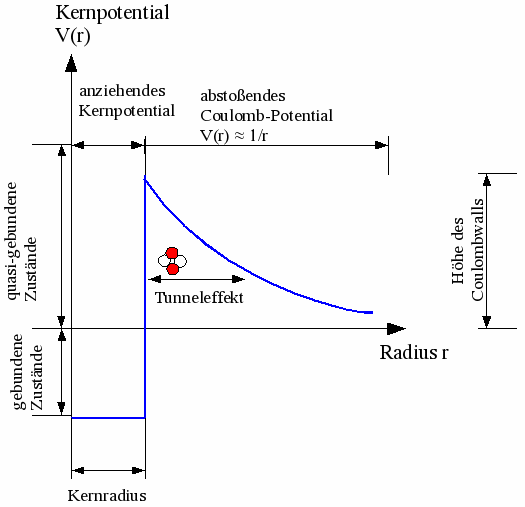
\includegraphics[width=0.7\textwidth]{images/coulomb.png}\\
		\footnotesize\sffamily\textbf{Quelle:} Wikipedia \cite{wiki:alpha}
	\end{tabular}
	\caption{Coulombwall}
    \label{fig:coulombwall}
\end{figure}
Nach den Gesetzen der klassischen Mechanik ist es nicht möglich, dass das Alphateilchen den Coulombwall überwindet, da die Höhe des Walls die Energie des Teilchens übertrifft. Daher wäre das Alphateilchen, klassisch betrachtet, stabil an den Kern gebunden (deswegen bezeichnet man diesen Zustand als \textbf{metastabil}). Jedoch, mit einer gewissen Wahrscheinlichkeit, bedingt durch die Halbwertszeit des Zerfalls, verlässt das Teilchen den Mutternkern unter Ausnutzung des quantenmechanischen Tunneleffekts, der einem Teilchen erlaubt, eine endlich lange und endlich hohe Energiebarriere mit einer gewissen Wahrscheinlichkeit durchzudringen, auch wenn klassisch seine Energie dafür nicht ausreicht.\\ \\
Nach dem Zerfall verbleibt der Atomkern in angeregtem Zustand. Der nachfolgende Übergang des Kerns vom angeregten in den Grundzustand erfolgt unter Aussendung von Gammastrahlung.\\ \\
Da beim Zerfall außerdem die Kernladungszahl um zwei Einheiten abnimmt, sich aber die Anzahl der Elektronen in der Elektronenhülle unverändert bleibt, liegt beim entstehenden Tochteratom zunächst ein Elektronenüberschuss vor, der wiederum durch Wechselwirkung mit der umgebenden Materie und anschließenden Verlust der überschussigen Elektronen ausgeglichen wird.
\subsubsection{$\beta$-Strahlung \cite{blauesBuch}, \cite{wiki:beta}}
Unter dem $\beta$-Zerfall versteht man alle Zerfallsmöglichkeiten eines Kerns, bei denen die Massenzahl $A$ konstant bleibt, und die Kernladungszahl $Z$ sich um eine Einheit ändert. Gleichzeitig entsteht ein Antineutrino bzw. Neutrino. Je nach Art der emittierten Teilchen unterscheidet man drei Arten:
\begin{description}
	\item[Beta-Minus-Zerfall ($\beta^{-}$)] \hfill \\Bei dieser Art wird ein Elektron abgestrahlt.
\begin{equation*}
\ce{^{A}_{Z}X} \rightarrow \ce{^{A}_{Z+1}Y} + e^{-}+ \overline{\nu}_e
\end{equation*}
Dabei zerfallen Nuklide mit einem Neutronenüberschuss über den $\beta^{-}$-Prozess, sodass sich ein Neutron in ein Proton umwandelt und dabei ein Elektron sowie ein Elektron-Antineutrino aussendet. Das Elektron und das Antineutrino verlassen den Atomkern, da diese Leptonen sind und sich nicht der starken Wechselwirkung unterliegen. Nun befindet sich im Kern ein Neutron wenige und ein Proton mehr, wodurch sich die Kernladungszahl $Z$ sich um $1$ erhöht und die Massenzahl $A$ konstant bleibt. 
    \item[Beta-Plus-Zerfall ($\beta^{+}$)] \hfill \\ Bei dieser Art wird ein Positon abgestrahlt.
\begin{equation*}
\ce{^{A}_{Z}X} \rightarrow \ce{^{A}_{Z-1}Y} + e^{+}+ \nu_e
\end{equation*}
Diese Art tritt bei protonenreichen Nukliden auf: ein Proton wird in ein Neutron umgewandelt und es entstehen dabei ein Positron und ein Elektron-Neutrino. Die Massenzahl des Kerns bleibt unverändert, die Kernladungszahl verringert sich um $1$.
	\item[Der Elektroneneinfang] \hfill \\Dabei fängt sich der Kern ein Elektron aus der Hülle ein; folglich wandelt sich ein Proton in ein Neutron und Neutrino um und erniedrigt die Kernladungszahl um eine Einheit. Dieser Prozess ist energetisch möglich, weil die Massen des Mutterkerns und Elektrons größer sind als die des Tochterkerns.
\end{description}
\subsubsection{$\gamma$-Strahlung \cite{wiki:gamma}}
$\gamma$-Strahlung entsteht dann, wenn sich nach einem Alpha- oder Betazerfall der zurückbleibende Kern sich in einem angeregten Zustand befindet und dann in einen weniger hoch angeregten oder den Grundzustand übergeht. Dabei wird Energie in Form von Gammastrahlung frei. Anders als bei den vorherigen Strahlungsarten zerfällt hierbei der Kern nicht, die Anzahl seiner Neutronen und Protonen bleibt erhalten.\\ \\
Bei den Gammastrahlen handelt es sich um elektromagnetische Wellen bzw. Photonen.
\subsection{Motivation des Versuchs}
Die elektromagnetische Strahlung einer radioaktiven Quelle ist isotrop, d.h. die Winkelverteilung der emittierten Strahlen ist isotrop.\\ \\
In diesem Versuch werden die Winkelkorrelationsfunktion und Anisotropie zweier korrelierten Gamma-Strahlen von radioaktivem $^{60}\ce{Ni}$ untersucht. Bei diesem Kaskadenzerfall sind die Emissionsrichtungen der zwei Gammastrahlen nicht unabhängig voneinander, es besteht ein Zusammenhang (Winkelkorrelation) \cite{web:korrelation}. Die Anisotropie ist die Abweichung einer Winkelkorrelation von einer isotropen Winkelverteilung.
\subsection{Erzeugung von $\gamma$-Strahlen}
Um Gammastrahlung zu erzeugen, wird in diesem Versuch (instabiles) $^{60}\ce{Co}$ verwendet. Das zerfällt zu dem stabilen $^{60}\ce{Ni}$ (siehe Abbildung \ref{fig:cobalt}).
\begin{figure}[H]
	\centering
	\begin{tabular}{@{}r@{}}
		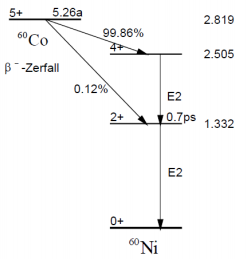
\includegraphics[width=0.45\textwidth]{images/cobalt.PNG}\\
		\footnotesize\sffamily\textbf{Quelle:} Blaues Buch \cite{blauesBuch}
	\end{tabular}
	\caption{Zerfallsschema für Cobalt-60}
    \label{fig:cobalt}
\end{figure}
Mit einer Übergangswahrscheinlichkeit von $\unit[99.86]{\%}$ findet ein Beta-Minus-Zerfall nach folgender Gleichung statt:
\begin{equation*}
\ce{^{60}_{27}X} \rightarrow \ce{^{60}_{28}Y} + e^{+}+ \overline{\nu_e}
\end{equation*}
Bei diesem Zerfall übergeht $\ce{^{60}Co}$ zunächst in einenen angeregten $\ce{^{60}Ni}$-Kern, der dann anschließend durch kurze hintereinandere Aussendung zweier Gammaquanten (Energie jeweils $\unit[1173]{keV}$ bzw. $\unit[1332]{keV}$) in den Grundzustand übergeht. Diese beiden Gammaquanten stellen die Grundlage für die Winkelkorrelationsmessungen dieses Versuches dar.
\subsection{Winkelkorrelation von Gammastrahlung}
Isotropie bzw. Anisotropie bezeichnet die Unabhängigkeit bzw. Abhängigkeit der Intensität der elektromagnetischen Strahlung (Gammastrahlung) vom Emissionswinkel bezüglich einer ausgezeichneten Richtung.\\ \\
Damit elektromagnetische Strahlung bei einem Übergang von einem Zustand mit Spin $J_1$ in einen Zustand mit Spin $J_2$ isotrop erfolgt, müssen die nachfolgenden Bedigungen erfüllt sein:
\begin{itemize}
\item die $2J_1 + 1$ Unterzustände mit verschiedenen magnetischen Quantenzahlen $m$ sind gleich besetzt
\item alle möglichen Übergänge zwischen den Zuständen $(J_1, m_1)$ und $(J_2, m_2)$ wurden beobachtet
\end{itemize}
Betrachte als Beispiel den Übergang zwischen dem Zustand $J_1=1$ und dem Grundzustand $J_2=0$. Dabei ist $J_1$ dreifach entartet mit magnetischen Quantenzahlen $m_1=+1, 0, -1$, der untere Zustand mit $m_2=0$, also gibt es drei mögliche Dipolübergänge mit
\begin{equation*}
\Delta m=m_1-m_2=+1, 0, -1
\end{equation*}
Für diese Übergänge leitet man aus der Optik die Wahrscheinlichkeiten her, mit denen sie eintreffen können:
\begin{equation*}
W_+ d\Omega=\frac{3}{16} \pi (1 + \cos^2{\theta})
\end{equation*}
\begin{equation*}
W_0 d\Omega=\frac{3}{8} \pi \sin^2{\theta}
\end{equation*}
\begin{equation*}
W_- d\Omega=\frac{3}{16} \pi (1 + \cos^2{\theta})
\end{equation*}
wobei $\theta$ der Winkel zwischen der Emissionsrichtung und der $z$-Achse, die als Quantisierungsachse gewählt ist, die beliebig sein kann.\\ \\
Die einzelnen Übergangswahrscheinlichkeiten $W_i$ sind nicht isotrop, die Summe davon ist jedoch isotrop, sofern alle Zustände gleichbesetzt sind:
\begin{equation*}
W_G=\sum\limits_{i} W_i d\Omega=\frac{3}{4} \pi d\Omega
\end{equation*}
Weil die Energieauflösung der im Versuch eingesetzten NaJ-Detektoren nicht klein genug ist, lassen sich die Übergänge der einzelnen Unterzustände nicht direkt auflösen - im Versuch wird nur die Gesamtwahrscheinlichkeit $W_G$ gemessen.\\ \\
Eine Anisotropie kann also nur dadurch gemessen werden, indem die Gleichbesetzung der Unterzustände aufgehoben wird. Dafür gibt es zwei Methoden: Polarisation der Kerne und Winkelkorrelation (Beobachtung von Zerfallskaskaden), letztere werden wir in diesem Versuch verwenden.\\ \\
Bei Winkelkorrelationsexperimenten entsteht die Anisotropie bei anfänglicher Gleichverteilung \emph{durch gleichzeitige Messung von zwei Übergängen}, z.B. ein $\beta$-Teilchen und ein nachfolgendes $\gamma$-Quant des Tochterkerns oder zwei $\gamma$-Quanten, wenn der Übergang in den Grundzustand über ein oder mehrere Zwischenzustände erfolgt. Durch gleichzeitige Beobachtung von zwei Übergängen wird die Gleichbesetzung bezüglich einer beliebigen Quantisierungsachse aufgehoben.\\ \\
Aus dem differentiellen Wirkungsquerschnitt (in anderen Worten, der Wahrscheinlichkeit) für die gleichzeitige Emission zweier $\gamma$-Quanten einer Kaskade in Abhängigkeit des Winkels $\theta$ zwischen den Emissionsrichtungen, lassen sich für die $\gamma$-Strahlung von $\ce{^{60}Co}$ (Quadrupolstrahlung) die zu bestimmende Korrelationsfunktion $K(\theta)$ und die Anisotropie $An$ ableiten:
\begin{eqnarray}
\label{eq:korrelation1}
K(\theta)&=&1+a_2 \cos^2{\theta} + a_4 \cos^4{\theta}\\
\label{eq:korrelation2}
An&=&K(180^{\circ}) - 1
\end{eqnarray}
Die unbekannten Koeffizienten $a_2$ und $a_4$ sollen experimentell aus der Korrelationsfunktion und der Anisotropie bestimmt werden. Die theoretischen Werte sind entsprechend $a_2=\frac{1}{8}$ und $a_4=\frac{1}{24}$.\\ \\
Die Korrelationsfunktion $K$ ist definiert als:
\begin{equation}
\label{eq:korrelation3}
K(\theta)=\frac{d \sigma (\theta)}{d \Omega} / \frac{d \sigma (90^{\circ})}{d \Omega}
\end{equation}
wobei $\frac{d \sigma}{d \Omega}$ den differentiellen Wirkungsquerschnitt bezeichnet.\\ \\
Desweiteren besteht zwischen dem differentiellen Wirkungsquerschnitt und der Zählrate $N$, die wir im Versuch messen werden, der folgende Zusammenhang:
\begin{equation}
\label{eq:korrelation4}
\sigma=f \cdot N
\end{equation}
Durch Einsetzen von \ref{eq:korrelation4} in \ref{eq:korrelation3} erhalten wir:
\begin{equation}
\label{eq:korrelation5}
K(\theta)=\frac{N(\theta)}{N(90^{\circ})}
\end{equation}
\subsection{Koinzidenzmessung}
Koinzidenzmessung bedeutet die Feststellung, dass zwei oder mehrere Ereignisse innerhalb einer bestimmten, vorgegebenen Zeit, der Koinzidenzauflösungszeit, stattgefunden haben.
\subsubsection{Koinzidenzschaltbild}
Blockschaltbild \ref{fig:koinzidenzschaltbild} zeigt den Aufbau eines Experiments zur Messung der Koinzidenz zweier Ereignisse in verschiedenen Detektoren. Das Signal gelangt zunächst zum Detektor (verwendet man Szintillatoren, wie in diesem Versuch der Fall ist, so werden jegliche Signalvorverstärker und -verstärker weggelassen). Nach der erforderlichen Zeitauflösung werden die Diskriminatoren ausgesucht, die Signale diskriminieren, also entscheiden welche Signale als Ereignisse gemessen werden sollen.
\begin{figure}[H]
	\centering
	\begin{tabular}{@{}r@{}}
		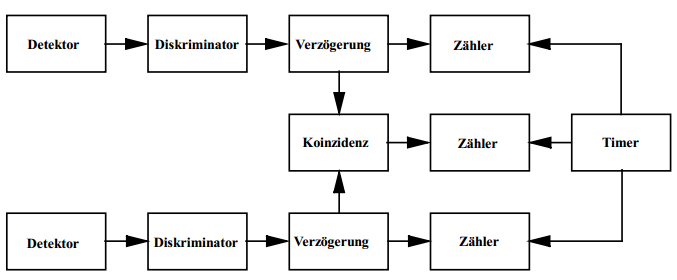
\includegraphics[width=0.7\textwidth]{images/koinzidenzmessung.PNG}\\
		\footnotesize\sffamily\textbf{Quelle:} Blaues Buch \cite{blauesBuch}
	\end{tabular}
	\caption{Koinzidenzschaltbild}
    \label{fig:koinzidenzschaltbild}
\end{figure}
Dann werden die in digitalen Impulsen umgewandelten Signale an die Verzögerungseinheiten geleitet, die dafür sorgen, dass eventuell vorhandene Laufzeitdifferenzen der Signale durch die variablen Verzögerungen sich ausgleichen und somit Signale physikalisch gleichzeitiger Ereignisse auch zur gleichen Zeit an die Koinzidenz gelangen.
\subsubsection{Aufbau des NaJ-Szintillations-Detektoren}
Die Wirkungsweise des Detektors beruht darauf, dass anorganische Substanzen wie NaJ von ionisierender Strahlung zur Emission von Licht angeregt werden. Beispielsweise rufen $\alpha$-Teilchen beim Auftreffen auf dem NaJ-Schirm Lichtblitze hervor, die man in frühen Tagen einfach beobachtet und gezählt hat.\\ \\
Heutzutage wird der Szintillator direkt vor der Photokathode eines Sekundärelektronenvervielfachers (SEV) gebracht. Dieser Aufbau ist unter dem Namen Photomultiplier bekannt. Die Photonen lösen dort durch den Photoeffekt Elektronen aus, die vervielfacht werden, indem sie durch elektrische Felder beschleunigt und auf weitere Elektroden (sog. Dynoden) gelenkt werden, wo jedes Elektron weitere erzeugt. Auf dieser Weise ist der Elektronenstrom beträchtlich verstärkt (um Verstärkungsfaktoren von bis zu $10^6$) worden.\\ \\
Das mit Thailium dotierte NaJ-Kristall sorgt dafür, dass einfallende Gammastrahlung durch Wechselwirkungsprozesse Sekundär- bzw. Tertiärelektronen erzeugt, die dann das NaJ-Kristall zur Photonenemission anregen.\\ \\
Szintillatoren sind durch folgende Größen charakterisiert:
\begin{enumerate}
\item Absolute Szintillationsempfindlichkeit S - gibt den Bruchteil der im Szintillator deponierten Energie $E$ an
\item Lage des Emissionsspektrums
\item Lichtausbeute/die spezifische Lichtausbeute - die gesamte vom Szintillator abgestrahlte Energie
\item Zerfallszeit - mittlere Lebensdauer $\tau$ der angeregten Emissionszentren
\end{enumerate}
\section{Überlegungen zum Versuch}
\subsection{Aufbau}
Im Versuch wird ein $\gamma$-Strahler verwendet bei dem wie bereits erwähnt $^{60}\ce{Co}$ in $^{60}\ce{Ni}$ zerfällt. Zur Detektion der $\gamma$-Quanten werden zwei NaJ-Szintillations-Detektoren verwendet, von denen einer auf eine feste Position gestellt ist und der andere in einem Winkel von $90^\circ$, $135^\circ$ und $180^\circ$ dazu aufgestellt wird. Die Detektoren sind gemäß dem Koinzidenzschaltbild angeschlossen. Diese Schaltung soll sicherstellen, dass die gleichzeitig detektierten Ereignisse auch (mit einer gewissen Wahrscheinlichkeit) aus dem selben Zerfallsprozess stammen.\\
Man könnte auf den Gedanken kommen eine möglichst aktive Probe zur Messung zu verwenden, um so die Messzeit gering zu halten, was allerdings nicht ratsam wäre. Der Grund dafür ist, dass die Anzahl der zufällig in einem Intervall stattfindenden Zerfälle (zufällige Koinzidenzen) quadratisch mit der Aktivität zunimmt, während die echten Koinzidenzen nur linear mit der Aktivität zusammenhängen. Dabei gilt für das Verhältnis aus echten ($N_K$) und zufälligen Koinzidenzen ($N_Z$):
\begin{equation}
\label{eq:aufloesungszeit}
\frac{N_K}{N_Z} \approx \frac{1}{\tau_A \cdot A}
\end{equation}
wobei $\tau_A$ die Auflösungszeit und $A$ die Aktivität bezeichnen.\\ \\
Die Auflösungszeit soll möglichst gering gehalten werden. Somit lässt sich mit dieser Gleichung die maximale Aktivität bestimmt werden, wenn ein gewisses Verhältnis eingehalten werden soll.

\subsection{Durchführung}
Neben den zufälligen Koinzidenzen kann die Messung auch verfälscht werden dadurch, dass in beliebigen Richtungen abgestrahlte Photonen an den Detektoren oder Halterungen eine Compton-Streuung erfahren und dann in den Zähler geraten. Die Mehrheit dieser Ereignisse kann aber unterdrückt werden, indem man die Diskriminatoren auf $60 \%$- $70 \%$ des Photopeaks einstellt, da die Streuung mit einem Energieverlust einhergeht. Um nicht zu viele der tatsächlichen Koinzidenzen zu unterdrücken, darf die Schwelle aber auch nicht zu hoch gewählt werden.\\
Es werden drei Messreihen durchgeführt, eine für jede Position des Szintillators. Eine Messung dauert genau $\unit[400]{s}$ und wird einmal wiederholt.\\
Um die Anzahl der zufälligen Koinzidenzen $N_Z$ festzustellen, werden die Delay-Einheiten zwischen Detektoren und Koinzidenzenstufe auf maximale Verzögerung ($2 \cdot \unit[66]{ns}$) eingestellt. Somit kommen die Koinzidenzen verzögert an die Koinzidenzenstufe und werden nicht mehr registriert. Was übrig bleibt sind die zufälligen Koinzidenzen. Die Anzahl dieser zufälligen Koinzidenzen muss nun von der Anzahl der gesamten Koinzidenzen abgezogen werden. Darüber hinaus gibt es noch eine Hintergrundstrahlung, welche berücksichtigt werden muss. Dazu werden am Ende noch zwei Messreihen ohne Probe durchgeführt, aus diesen erhält man einen Wert für die mittlere Anzahl an Hintergrund-Photonen und einen Wert für die zufälligen Koinzidenzen in der Hintergrundstrahlung. Diese müssen ebefalls von den Ergebnissen der Messreihen mit Probe abgezogen werden.

\section{Auswertung}
\subsection{Verlauf des Versuchs}
Zunächst bauten wir, unterstützt vom Betreuer, die Koinzidenzschaltung auf und kalibrierten die Detektoren so, dass die Anzahl der Koinzidenzen bei einer $\unit[400]{s}$ langen Messung zwischen 160 und 200 lag.\\ \\
Nachfolgend stellten wir die Diskriminatoren auf ungefähr $\frac{2}{3}$ des Photopeaks ein. Mithilfe eines Oszilloskops beobachteten wir die Impulse der Detektoren und stellten anhand des Spektrums sicher, dass beide (fast) gleich eingestellt waren. Ein maximaler Impuls bedeutet, dass ein $\gamma$-Quant registriert wurde. War der Impuls kleiner, so wurde das $\gamma$-Quant vor dem Eintritt in den Detektor gestreut, d.h. er gab einen Teil seiner Energie ab. Durch die Diskriminatoreinstellung wird sichergestellt, dass möglichst viele ungestreute $\gamma$-Quanten gezählt werden. Die richtige Einstellung der Diskriminatoren gestaltete sich schwierig, da die registrierten Impulse schwach und der Photopeak am Oszilloskop schwer erkennbar waren. Die Messzeit war auf $\unit[400]{s}$ eingestellt.\\ \\
Wir führten dann die Messungen durch, wobei die Zählraten der jeweiligen Detektoren und die Anzahl der Koinzidenzen notiert wurden.\\ \\
Zur Abschätzung der Untergrundstrahlung wurde am Anfang eine Messung ohne Probe durchgeführt. Es wurde keine Koinzidenz gemessen.\\ \\
Desweiteren wurden zur Bestimmung der zufälligen Koinzidenzen zwei weitere Messungen mit Probe gemacht, wofür wir die maximale Verzögerung der Delay-Einheiten (je $\unit[66]{ns}$) und die Detektoren in einem Winkel $180^{\circ}$ zueinander einstellten. Es wurden wieder keine zufälligen Koinzidenzen gemessen.\\ \\
Weitere Messungen ohne Delay fanden nacheinander für die Winkel $180^{\circ}$, $135^{\circ}$ und $90^{\circ}$ statt, wobei für jeden Winkel 2 Messungen erfolgten. Es gab 2 weitere solche Durchgänge. Tabelle \ref{tab:measurements} fasst alle Messdaten zusammen.
\begin{table}[H]
\centering
\begin{tabular}{c|c|c|c|c|c}
Messreihe & Winkel & Delay & $N_1$ & $N_2$ & $N_k$ (Koinzidenzen)\\
\hline
& Untergrundmessung & nein & \numprint{1010} & 764 & 0\\
\hline
1 & \multirow{6}{*}{$90^{\circ}$} & nein & \numprint{23430} & \numprint{22391} & 50\\
1 & & nein & \numprint{23547} & \numprint{22271} & 43\\
2 & & nein & \numprint{23689} & \numprint{22491} & 41\\
2 & & nein & \numprint{23501} & \numprint{22420} & 47\\
3 & & nein & \numprint{24035} & \numprint{22768} & 52\\
3 & & nein & \numprint{23752} & \numprint{22538} & 45\\
\hline
1 & \multirow{6}{*}{$135^{\circ}$} & nein & \numprint{22267} & \numprint{22430} & 44\\
1 & & nein & \numprint{22078} & \numprint{22323} & 47\\
2 & & nein & \numprint{22239} & \numprint{22634} & 60\\
2 && nein & \numprint{22184} & \numprint{22587} & 36\\
3 & & nein & \numprint{22530} & \numprint{22952} & 56\\
3 & & nein & \numprint{22214} & \numprint{22739} & 52\\
\hline
- & \multirow{8}{*}{$180^{\circ}$} & ja & \numprint{20596} & \numprint{21918} & 0\\
- & & ja & \numprint{20470} & \numprint{22443} & 0\\
1 & & nein & \numprint{20516} & \numprint{22370} & 42\\
1 && nein & \numprint{20392} & \numprint{22519} & 48\\
2 & & nein & \numprint{20151} & \numprint{22847} & 37\\
2 & & nein & \numprint{20236} & \numprint{22375} & 50\\
3 && nein & \numprint{20517} & \numprint{22478} & 48\\
3 & & nein & \numprint{20851} & \numprint{22473} & 47
\end{tabular}
\caption{Zusammenfassung der Messergebnisse}
\label{tab:measurements}
\end{table}
\subsection{Korrektur der Messdaten}
Vor der weiteren Auswertung müssen die Werte der Untergrundstrahlung von den Messwerten des jeweiligen Detektors substrahiert werden.\\ \\
Weiterhin müssen die Koinzidenzraten durch das Produkt der zugehörigen Einzelraten dividiert werden, um Fehler durch eventuell wanderende Schwellen, mangelhafte Justierung und unterschiedlichen Raumwinkeln zu eleminieren, welche die reduzierte Koinzidenzrate $\tilde{n}$ ergibt:
\begin{equation*}
\tilde{n}=\frac{N_k}{N_1 \cdot N_2}
\end{equation*}
Abschließend muss von den reduzierten Koinzidenzraten $\tilde{n}$ die reduzierte zufällige Koinzidenzrate $\tilde{n}_z$ substrahiert werden. Weil bei der Messung mit Delay (vgl. Tabelle \ref{tab:measurements}) keine Koinzidenz $N_k$ gemessen wurde, beträgt $\tilde{n}_z=0$.\\ \\
Tabelle \ref{tab:correctedCoincidences} listet die korrigierten reduzierten Koinzidenzraten auf, die für die weitere Auswertung verwendet werden.
\begin{table}[H]
\centering
\begin{tabular}{c|c|c}
Messreihe & Winkel $\theta$ & korrigierte reduzierte Koinzidenzrate $\tilde{n}$\\
\hline
1 & \multirow{6}{*}{$90^{\circ}$} & $9.53 \cdot 10^{-8}$\\
1 & & $8.19 \cdot 10^{-8}$\\
2 & & $7.69 \cdot 10^{-8}$\\
2 & & $8.92 \cdot 10^{-8}$\\
3 & & $9.50 \cdot 10^{-8}$\\
3 & & $8.40 \cdot 10^{-8}$\\
\hline
1 & \multirow{6}{*}{$135^{\circ}$} & $8.80 \cdot 10^{-8}$\\
1 & & $9.53 \cdot 10^{-8}$\\
2 & & $1.19 \cdot 10^{-7}$\\
2 & & $7.18 \cdot 10^{-8}$\\
3 & & $1.08 \cdot 10^{-7}$\\
3 & & $1.02 \cdot 10^{-7}$\\
\hline
1 & \multirow{6}{*}{$180^{\circ}$} & $9.15 \cdot 10^{-8}$\\
1 & & $1.04 \cdot 10^{-7}$\\
2 & & $8.03 \cdot 10^{-8}$\\
2 & & $1.10 \cdot 10^{-7}$\\
3 & & $1.04 \cdot 10^{-7}$\\
3 & & $1.00 \cdot 10^{-7}$\\
\end{tabular}
\caption{Korrigierte reduzierte Koinzidenzraten $\tilde{n}$}
\label{tab:correctedCoincidences}
\end{table}
Um die weitere Auswertung zu vereinfachen, setzen wir in Gleichung \ref{eq:korrelation1} für die bereits bekannten Winkeln $\cos(135^{\circ})=-\frac{\sqrt{2}}{2}$ und $\cos(180^{\circ})=-1$ ein:
\begin{equation*}
\left\{
\begin{aligned}
K(135^{\circ})&=1+\frac{1}{2}a_2+\frac{1}{4}a_4\\
K(180^{\circ})&=1+a_2+a_4
\end{aligned}
\right.
\end{equation*}
Das Gleichungssystem ist lösbar und wir bestimmen die Koeffizienten $a_2$, $a_4$ zu:
\begin{equation}
\label{eq:koeffizientenEinfach}
\begin{aligned}
a_2&=4K(135^{\circ})-K(180^{\circ})-3\\
a_4&=2K(180^{\circ}) - 4K(135^{\circ}) + 2
\end{aligned}
\end{equation}
\subsection{Auswertung nach der 1. Methode}
Nach dieser Methode werden alle zu einem Winkel gehörenden Koinzidenzen aus Tabelle \ref{tab:correctedCoincidences} zusammenaddiert, Tabelle \ref{tab:addedCoincidence} stellt das Endergebnis dar.
\begin{table}[H]
\centering
\begin{tabular}{c|c}
Winkel & $\tilde{n}$\\
\hline
$90^{\circ}$ & $5.22 \cdot 10^{-7}$\\
$135^{\circ}$ & $5.84 \cdot 10^{-7}$\\
$180^{\circ}$ & $5.89 \cdot 10^{-7}$\\
\end{tabular}
\caption{Zusammenaddierte Koinzidenzraten}
\label{tab:addedCoincidence}
\end{table}
\subsubsection{Koeffizienten- und Anisotropiebestimmung}
Aus den Gleichungen \ref{eq:koeffizientenEinfach} und \ref{eq:korrelation2} und Einsetzen der Koinzidenzraten der Tabelle \ref{tab:addedCoincidence} können jeweils die Koeffizienten $a_2$, $a_4$ und die Anisotropie bestimmt werden.\\ \\
Zunächst sind die Korrelationsfunktionen $K(135^{\circ})$, $K(180^{\circ})$ mithilfe der Gleichung \ref{eq:korrelation5} zu bestimmen:
\begin{equation*}
\begin{aligned}
K(135^{\circ})&=\frac{\tilde{n}(135^{\circ})}{\tilde{n}(90^{\circ})}=\frac{5.84 \cdot 10^{-7}}{5.22 \cdot 10^{-7}}=1.118\\
K(180^{\circ})&=\frac{\tilde{n}(180^{\circ})}{\tilde{n}(90^{\circ})}=\frac{5.89 \cdot 10^{-7}}{5.22 \cdot 10^{-7}}=1.128\\
\end{aligned}
\end{equation*}
Nun lassen sich $a_2$, $a_4$ und die Anisotropie $An$ bestimmen:
\begin{equation*}
\begin{aligned}
a_2&=4K(135^{\circ})-K(180^{\circ})-3=4 \cdot 1.118-1.128-3=0.344\\
a_4&=2K(180^{\circ}) - 4K(135^{\circ}) + 2=2 \cdot 1.128 - 4 \cdot 1.118 + 2=-0.216\\
An&=K(180^{\circ}) - 1=1.128-1=0.128
\end{aligned}
\end{equation*}
\subsubsection{Fehlerrechnung}
Die am Detektor registrierten Zählraten $N_j$ ($j = 1,2,K$) sind poissonverteilt, daher ergibt sich für die Zählraten ein statistischer Fehler mit $\sigma_{N_j}=\sqrt{N_j}$. \\ \\
Um die Unsicherheiten von $a_2$, $a_4$ und $An$ zu bestimmen, werden wir nun alle im vorherigen Abschnitt durchgeführten Rechenschritte zurückverfolgen und jeweils den statistichen Fehler fortpflanzen.
\begin{description}
\item[Fehler der um die Untergrundsmessung korrigierten Zählraten] Die gemessenen Zählraten wurden unter Berücksichtigung der Untergrundstrahlung korrigiert, indem der am entsprechenden Detektor registrierte Untergrundsmessung $N_{U,j}$ davon substrahiert wurde. Die Gaußsche Fehlerfortpflanzung liefert für den Fehler des um den Untergrund korrigierten Wertes:
\begin{equation*}
\sigma_{N_{j,k}}=\sqrt{\sigma^2_{N_j}+\sigma^2_{N_{U,j}}}
\end{equation*}
mit $j=1,2,K$ jeweils für Detektor 1, 2 und Koinzidenzen und $\sigma_{N_j}=\sqrt{N_j}$.
\item[Fehler der korrigierten reduzierten Koinzidenzrate $\tilde{n}$] Nach der Korrektur um den Untergrundmessungswert, wurde die korrigierte reduzierte Koinzidenzrate $\tilde{n}$ berechnet:
\begin{equation*}
\tilde{n}=\frac{N_k}{N_1 \cdot N_2}
\end{equation*}
Da $N_k$, $N_1$ und $N_2$ jeweils mit statistischem Fehler behaftet sind, ergibt sich der statistische Fehler $\sigma_{\tilde{n}}$ wiederum aus der Gaußschen Fehlerfortpflanzung:
\begin{equation*}
\sigma_{\tilde{n}}=\sqrt{\left(\frac{1}{N_1 N_2}\right)^2 \sigma^2_{N_k}+\left(\frac{-N_k}{N_1^2 N_2}\right)^2 \sigma_{N_1}^2+\left(\frac{-N_k}{N_1 N_2^2}\right)^2 \sigma_{N_2}^2}
\end{equation*}
\item[Fehler der um zufällige Koinzidenzen korrigierten Zählraten] Da bei der Messung mit an der Koinzidenzschaltung eingestelltem Delay keine zufälligen Koinzidenzen gemessen werden konnten, gibt es an dieser Stelle keinen Fehler zu berücksichtigen.
\item[Fehler der Summe der korrigierten Koinzidenzraten] Alle zu einem Winkel gehörenden Koinzidenzraten wurden addiert. Der Fehler dieser Summe beträgt:
\begin{equation*}
\sigma_{\tilde{n}_M(\Theta)}=\sqrt{\sum_{i=1}^6 \sigma^2_{\tilde{n}_i(\Theta)}}
\end{equation*}
wobei $\sigma_{\tilde{n},i}(\Theta)$ den Fehler der $i$. gemessenen, korrigierten, reduzierten Koinzidenzrate $\tilde{n}$ bezeichnet.
\item[Fehler der Korrelationsfunktion] Die Korrelationsfunktion wurde nach Gleichung \ref{eq:korrelation5} bestimmt, deren Fehler ergibt sich wieder mit der Gaußschen Fehlerfortpflanzung:
\begin{eqnarray*}
\sigma_{K(\Theta)}&=&\sqrt{\left(\frac{\partial K(\Theta)}{\partial \tilde{n}(\Theta)}\right)^2 \sigma^2_{\tilde{n}_M(\Theta)}+\left(\frac{\partial K(\Theta)}{\partial \tilde{n}(90^{\circ})}\right)^2 \sigma^2_{\tilde{n}_M(90^{\circ})}}\\
&=&\sqrt{\left( \frac{1}{\tilde{n}(90^{\circ})} \right)^2 \sigma^2_{\tilde{n}_M(\Theta)} + \left( \frac{- \tilde{n} (\Theta)}{\tilde{n}^2 (90^{\circ})} \right)^2 \sigma_{\tilde{n}_M(90^{\circ})}^2}
\end{eqnarray*}
\item[Fehler der Parameter $a_2$ und $a_4$]
\begin{equation*}
\sigma_{a_i}=\sqrt{\left(\frac{\partial a_i}{\partial K(135^{\circ})}\right)^2 \sigma^2_{K(135^{\circ})} + \left(\frac{\partial a_i}{\partial K(180^{\circ})}\right)^2 \sigma^2_{K(180^{\circ})}}
\end{equation*}
Wir erhalten jeweils für $a_2$ und $a_4$:
\begin{eqnarray*}
\sigma_{a_2}&=&\sqrt{\sigma^2_{K(180^{\circ})} + 16 \cdot \sigma^2_{K(135^{\circ})}}\\
\sigma_{a_4}&=&\sqrt{4 \cdot \sigma^2_{K(180^{\circ})} + 16 \cdot \sigma^2_{K(135^{\circ})}}
\end{eqnarray*}
Nach Einsetzen der Fehlerwerte der Korrelationsfunktion erhalten wir:
\begin{eqnarray*}
\sigma_{a_2}&=&0.388\\
\sigma_{a_4}&=&0.422
\end{eqnarray*}
\item[Fehler der Anisotropie] Die Anisotropie hatten wir anhand Gleichung \ref{eq:korrelation2} berechnet, der Fehler $\sigma_{An}$ ist deshalb:
\begin{equation*}
\sigma_{An}=\sigma_{K(180^{\circ})}=0.096
\end{equation*}
\end{description}
\subsubsection{Ergebnis}
Wir fassen die Parameter $a_2$, $a_4$, die Anisotropie und ihre Unsicherheiten zusammen:
\begin{eqnarray*}
a_2&=&0.344 \pm 0.388\\
a_4&=&-0.216 \pm 0.422\\
An&=&0.128 \pm 0.096
\end{eqnarray*}
\subsection{Auswertung nach der 2. Methode}
Nach dieser Methode werden die 3 Messreihen als unabhängig angesehen und getrennt ausgewertet. Dabei werden die 2 für jeden Winkel gemessenen Koinzidenzen gemittelt:
\begin{equation*}
\overline{n}=\frac{1}{2}(\tilde{n}_1(\Theta) + \tilde{n}_2(\Theta))
\end{equation*}
Tabelle \ref{tab:separatedCoincidence} zeigt die berechneten Koinzidenzraten für jeden Winkel der jeweiligen Messreihe.
\begin{table}[H]
\centering
\begin{tabular}{c|c|c}
Messreihe & Winkel $\theta$ & $\overline{n}$\\
\hline
\multirow{3}{*}{1} & $90^{\circ}$ & $8.86 \cdot 10^{-8}$\\
& $135^{\circ}$ & $9.16 \cdot 10^{-8}$\\
& $180^{\circ}$ & $9.77 \cdot 10^{-8}$\\
\hline
\multirow{3}{*}{2} & $90^{\circ}$ & $8.30 \cdot 10^{-8}$\\
& $135^{\circ}$ & $9.54 \cdot 10^{-8}$\\
& $180^{\circ}$ & $9.51 \cdot 10^{-8}$\\
\hline
\multirow{3}{*}{3} & $90^{\circ}$ & $8.95 \cdot 10^{-8}$\\
& $135^{\circ}$ & $1.05 \cdot 10^{-7}$\\
& $180^{\circ}$ & $1.02 \cdot 10^{-7}$\\
\end{tabular}
\caption{Korrigierte reduzierte Koinzidenzraten der jeweiligen Messreihen}
\label{tab:separatedCoincidence}
\end{table}
\subsubsection{Koeffizienten- und Anisotropiebestimmung}
Nachdem oben die Koinzidenzraten für jeden Winkel jedes Durchlaufs berechnet wurden, können nun die Koeffizienten und die Anisotropie analog zur 1. Methode bestimmt werden. Ein detailliertes Ausrechnen sei erspart, die Ergebnisse sind in Tabelle \ref{tab:auswertungMethode2} zu finden.
\begin{table}[H]
\centering
\begin{tabular}{c|c|c|c|c|c}
Messreihe & $K(135^{\circ})$ & $K(180^{\circ})$ & $a_2$ & $a_4$ & $An$ \\
\hline
1 & 1.034 & 1.103& 0.032 & 0.070 & 0.103\\
2 & 1.149 & 1.146 & 0.451 & -0.306 & 0.146\\
3 & 1.173 & 1.140 & 0.552 & -0.413 & 0.140\\
\hline
gemittelt & 1.119 & 1.129 & 0.345 & -0.216 & 0.129\\
\end{tabular}
\caption{Koeffizienten und Anisotropien der einzelnen Messreihen}
\label{tab:auswertungMethode2}
\end{table}
\subsubsection{Fehlerrechnung}
Die Fehler \emph{der um die Untergrundmessung korrigierten Zählraten}, \emph{der korrigierten reduzierten Koinzidenzraten $\tilde{n}$} und \emph{der um zufällige Koinzidenzen korrigerten Zählraten} wurden bereits bei der Fehlerrechnung der 1. Methode berechnet und können hier wiederverwendet werden.
\begin{description}
\item[Fehler des Mittelwertes der korrigierten Koinzidenzraten] Für jeden Winkel jedes Durchlaufs mittelten wir deren 2 korrigierten Koinzidenzraten $\tilde{n}(\Theta)$. Der Fehler des Mittelwerts $\sigma_{\overline{n}}$ muss deshalb durchgepflanzt werden:
\begin{eqnarray*}
\overline{n}&=&\frac{1}{2}(\tilde{n}_1(\Theta) + \tilde{n}_2(\Theta))\\
\Longrightarrow \sigma_{\overline{n}}&=&\sqrt{\left(\frac{\partial \overline{n}}{\partial \tilde{n}_1(\Theta)}\right)^2 \sigma^2_{\tilde{n}_1(\Theta)} + \left(\frac{\partial \tilde{n}}{\partial \tilde{n}_2(\Theta)}\right)^2 \sigma^2_{\tilde{n}_2(\Theta)}}\\
&=&\frac{1}{2} \sqrt{\sigma^2_{\tilde{n}_1(\Theta)} + \sigma^2_{\tilde{n}_2(\Theta)}}
\end{eqnarray*}
\item[Fehler der Korrelationsfunktion] Dieser berechnet sich analog wie bei der 1. Methode:
\begin{equation*}
\sigma_{K(\Theta)}=\sqrt{\left(\frac{1}{\overline{n}(90^{\circ})}\right)^2 \sigma^2_{\overline{n}(\Theta)} + \left(\frac{\overline{n}(\Theta)}{\overline{n}^2(90^{\circ})}\right)^2 \sigma^2_{\overline{n}(90^{\circ})}}
\end{equation*}
\item[Fehler der Parameter $a_2$, $a_4$ und Anisotropie] Völlig analog zur 1. Methode.
\item[Fehler des Mittelwertes der Parameter und der Anisotropie] Der Fehler des Mittelwertes ist die Standardabweichung dividiert durch die Wurzel aus der Anzahl der Messungen. Wir mittelten die Parameter $a_2$, $a_4$ und die Anisotropie von 3 Messreihen, deshalb berechnen sich die Fehler deren Mittelwerte wie folgt:
\begin{eqnarray*}
\sigma_{\overline{a_2}}&=&\sqrt{\frac{1}{6} \sum_{i=1}^3 (a_{2,i}-\overline{a_2})^2}\\
\sigma_{\overline{a_4}}&=&\sqrt{\frac{1}{6} \sum_{i=1}^3 (a_{4,i}-\overline{a_4})^2}\\
\sigma_{\overline{An}}&=&\sqrt{\frac{1}{6} \sum_{i=1}^3 (An_i-\overline{An})^2}
\end{eqnarray*}
\end{description}
\subsubsection{Ergebnis}
Tabelle \ref{tab:auswertungMethode2} wurde um die Unsicherheiten der Parameter $a_2$, $a_4$ und der Anisotropie erweitert:
\begin{table}[H]
\centering
\begin{tabular}{c|c|c|c|c|c|c|c|c}
Messreihe & $K(135^{\circ})$ & $K(180^{\circ})$ & $a_2$ & $\sigma_{a_2}$ & $a_4$ & $\sigma_{a_4}$ & $An$ & $\sigma_{An}$ \\
\hline
1 & 1.034 & 1.103 & 0.032 & 0.607 & 0.070 & 0.663 & 0.103 & 0.154\\
2 & 1.149 & 1.146 & 0.451 & 0.648 & -0.306 & 0.705 & 0.146 & 0.160\\
3 & 1.173 & 1.140 & 0.552 & 0.696 & -0.413 & 0.755 & 0.140 & 0.168\\
\hline
gemittelt & 1.119 & 1.129 & 0.345 & 0.159 & -0.216 & 0.146 & 0.129 & 0.013\\
\end{tabular}
\caption{Koeffizienten und Anisotropien der einzelnen Messreihen}
\label{tab:auswertungMethode2}
\end{table}
\subsection{Bestimmung der Auflösungszeit $\tau_A$}
Die Auflösungszeit der Koinzidenz $\tau_A$ bestimmen wir nach Gleichung \emph{7-104} aus dem blauen Buch \cite{blauesBuch}:
\begin{equation*}
\tau_A=\frac{N_Z}{N_1 N_2}=\unit[0]{s}
\end{equation*}
da wir keine zufälligen Koinzidenzen $N_Z$ ($N_Z=0$) gemessen haben.
Den Fehler $\sigma_{\tau_A}$ bestimmen wir durch Fehlerfortpflanzung:
\begin{eqnarray*}
\sigma_{\tau_A}&=&\sqrt{\left( \frac{\partial \tau_A}{\partial N_Z} \right)^2 \sigma^2_{N_z} + \left( \frac{\partial \tau_A}{\partial N_1} \right)^2 \sigma^2_{N_1} + \left( \frac{\partial \tau_A}{\partial N_2} \right)^2 \sigma^2_{N_2}}\\
&=&\sqrt{\left(\frac{1}{N_1 N_2}\right)^2 \sigma^2_{N_Z}+\left(\frac{-N_Z}{N_1^2 N_2}\right)^2 \sigma_{N_1}^2+\left(\frac{-N_Z}{N_1 N_2^2}\right)^2 \sigma_{N_2}^2}
\end{eqnarray*}
Wegen $N_Z=0$ folgt:
\begin{equation*}
\sigma_{\tau_A}=\frac{\sigma_{N_Z}}{N_1 N_2}
\end{equation*}
Weil $\sigma_{N_Z}=\sqrt{N_Z}=0$, ist $\sigma_{\tau_A}=0$. Also $\tau_A=\unit[0]{s}$.\\ \\
Dieses Ergebnis ist unmöglich, da die Detektoren immer eine Auflösungszeit $\tau_A > 0$ haben, innerhalb der erwartet wird, dass mehrere Ereignisse auftreten und registriert werden. Bei maximaler Verzögerung ($2 \cdot \unit[66]{ns}$) wurden jedoch keine zufälligen Koinzidenzen gemessen, was zu diesem absurden Ergebnis geführt hat. Die Messung der zufälligen Koinzidenzen hätte bei der Versuchsdurchführung so oft wiederholt werden müssen, bis zufällige Koinzidenzen festgestellt werden konnten.
\subsection{Diskussion der Ergebnisse und Vergleich beider Methoden}
Tabelle \ref{tab:comparison} vergleicht die Ergebnisse der 1. und 2. Methoden und die theoretischen Werte miteinander.
\begin{table}[H]
\centering
\begin{tabular}{c|c|c|c}
& 1. Methode & 2. Methode & theoretischer Wert\\
\hline
$a_2$ & $0.344 \pm 0.388$ & $0.345 \pm 0.159$ & 0.125\\
$a_4$ & $-0.216 \pm 0.422$ & $-0.306 \pm 0.146$ & 0.042\\
$An$ & $0.128 \pm 0.096$ & $0.146 \pm 0.013$ & 0.167\\
\end{tabular}
\caption{Vergleich der Methoden}
\label{tab:comparison}
\end{table}
Unsere Ergebnisse sind alle schlecht, da sie sehr stark von den theoretischen Werten abweichen. Die Unsicherheiten sind gegenüber der jeweiligen Werten sehr groß (z.B. bei der 1. Methode für $a_2$ und $a_4$ jeweils größer als $\unit[100]{\%}$ und $\unit[200]{\%}$).\\ \\
Die Theoriewerte liegen bei allen durch die 2. Methode bestimmten Parametern außerhalb der Fehlerbereiche.\\ \\
Die Fehlerbereiche sind bei der 1. Methode größer als bei der 2., die Werte jedoch fast gleich, da sie aus den gleichen Messdaten gewonnen wurden. Das bedeutet nicht, dass die 2. Methode bessere Ergebnisse liefert, schließlich liegt keine der Theoriewerten innerhalb deren Fehlerbereiche.\\ \\
Längere Messzeiten bzw. mehr Messreihen würden wahrscheinlich zu kleineren Fehlerbereichen bzw. präziseren Bestwerten führen.\\ \\
Desweiteren würden kleinere Fehlerbereiche in der 1. Methode darauf hinweisen, dass bei längerer Messdauer die Genauigkeit der Ergebnisse sich verbessern würde. Das ist nicht der Fall, da der Fehler viel größer ist. Es ist davon auszugehen, dass erst mit einer neuen Apparatur viel bessere Ergebnisse zu erzielen wären.
\bibliographystyle{acm}
\bibliography{lit}

\end{document}